\subsection{Finite fields and arithmetic circuits}
While computational models tipically operate over binary strings, that is, elements of 
\({\{0, 1\}}^*\), where \(*\) indicates Kleene's closure, we often want to interpret such strings 
as elements of some algebraic structure.
A \emph{field} is any set equipped with two binary operations, called addition
(denoted \(\oplus \)) and multiplication (denoted \(\otimes \)), which, in simple terms, have all
the nice properties of addition and multiplications over real numbers (\(\mathbb{R}\) is a field,
where \(\oplus \equiv +\) and \(\otimes \equiv \times \)).
The most common field used to represent bits is of course the \emph{boolean field} \(\mathbb{B}\),
where \(\oplus \equiv \textsc{xor}\) and \(\otimes \equiv \textsc{and}\).
Bit-strings of length \(n\) can be interpreted as elements of a \emph{finite field}
\(\mathbb{Z}_{q}\), where \(\oplus \) and \(\otimes \) are defined respectively as integer addition
and multiplication modulo \(q\), and \(q = p^k\), where \(p\) is a prime number and
\(k \in \mathbb{N}\).
Usually, either \(p = 2\) and \(k = n\), or \(p\) is some `big' prime number (\(\approx 2^n\)) and
\(k = 1\).
When the meaning is clear from the context, we will use \(+\) in place of \(\oplus \) and
omit \(\otimes \), like one would do with real numbers.
Sequences of operations over field elements and variables can be neatly represented by
\emph{arithmetic circuits}.
\begin{definition}[Arithmetic circuit]
	Given a field \(\mathbb{F}\), some \(n, m \in \mathbb{N}\), some constants
	\(a_{1, 1}, \dots, a_{m, n} \in \mathbb{F}\), and some variables \(x_1, \dots, x_n \) over
	\(\mathbb{F}\), an \emph{implicit arithmetic circuit} over \(\mathbb{F}\) is any formula:
	\begin{align*}
		 & \phi \equiv c                     &  & \textnormal{with \(c \in \mathbb{F}\)}
		\\
		 & \phi \equiv x                     &  & \textnormal{with \(x\) variable over
			\(\mathbb{F}\)}
		\\
		 & \phi \equiv \phi_1 \oplus \phi_2  &  & \textnormal{with \(\phi_1\) and \(\phi_2\)
			arithmetic
			circuits}
		\\
		 & \phi \equiv \phi_1 \otimes \phi_2 &  & \textnormal{with \(\phi_1\) and \(\phi_2\)
			arithmetic
			circuits}
		\\
		 & \phi \equiv \phi_1^c              &  & \textnormal{with \(c \in \mathbb{F}\) and
			\(\phi_1\) arithmetic
			circuit}
	\end{align*}
	An arithmetic circuit which does not contain multiplications and exponentiations by constants
	is called \emph{(explicit) arithmetic circuit}.
\end{definition}

\noindent Every arithmetic circuit can be represented by a Directed Acyclic Graph (DAG),
where the vertices are labeled either with a variable name (\emph{variable vertices}), a constant
from the field (\emph{constant vertices}) or one of the operations \(\oplus \)
(\emph{addition vertices}) and \(\otimes \) (\emph{multiplication vertices}, together with the
addition vertices are called \emph{operation vertices}).
With an analogy to digital circuits, vertices are also called \emph{gates}.
Only operation vertices have incoming edges, which must be exactly two, and represent the inputs of
the operation, while the outgoing edge will represent the result.
It is possible, without affecting the expressive power, to transform an implicit arithmetic circuit
into an explicit one by replacing exponentiations (multiplications) by some constant \(c\) with a
a sequence of \(c\) multiplications (additions)\footnote{On the other
	hand, such transformation does affect the succintness of some circuits (unrolling \(x^c\) or
	\(cx\) requires \(\BigO(2^c)\) space) and in turn their DAG representation.
	However, this won't be a problem for us.}.
\begin{example}\label{ex:circuit}
	Let's consider the following implicit arithmetic circuit over real numbers:
	\[\phi = x_{2}(x_{1}^{3} + 4x_{2} + 5)\]
	We can unroll it into an equivalent (explicit) arithmetic circuit:
	\[\widehat{\phi} = x_{2}(x_{1}x_{1}x_{1} + x_{2} + x_{2} + x_{2} + x_{2} + 5)\]
	And draw the associated DAG, which is shown in Figure~\ref{fig:example_dag}.
\end{example}
\begin{figure}
	\centering
	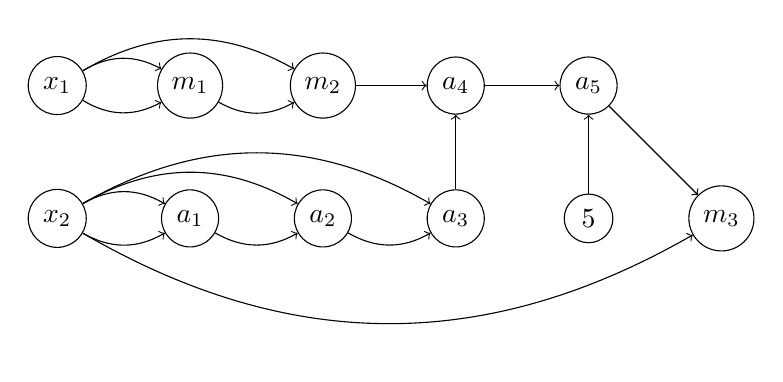
\begin{tikzpicture}[node distance={48pt}, node/.style = {draw, circle}]
		\node[node] (x1) {\(x_1\)};
		\node[node] (x2) [below of=x1] {\(x_2\)};
		\node[node] (m1) [right of=x1] {\(m_1\)};
		\node[node] (m2) [right of=m1] {\(m_2\)};
		\node[node] (a1) [right of=x2] {\(a_1\)};
		\node[node] (a2) [right of=a1] {\(a_2\)};
		\node[node] (a3) [right of=a2] {\(a_3\)};
		\node[node] (a4) [right of=m2] {\(a_4\)};
		\node[node] (a5) [right of=a4] {\(a_5\)};
		\node[node] (5) [below of=a5] {\(5\)};
		\node[node] (m3) [right of=5] {\(m_3\)};
		\draw[->] (x1) to [bend left] (m1);
		\draw[->] (x1) to [bend right] (m1);
		\draw[->] (x1) to [bend left] (m2);
		\draw[->] (m1) to [bend right] (m2);
		\draw[->] (x2) to [bend left] (a1);
		\draw[->] (x2) to [bend left] (a2);
		\draw[->] (x2) to [bend left] (a3);
		\draw[->] (x2) to [bend right] (a1);
		\draw[->] (a1) to [bend right] (a2);
		\draw[->] (a2) to [bend right] (a3);
		\draw[->] (m2) to (a4);
		\draw[->] (a3) to (a4);
		\draw[->] (a4) to (a5);
		\draw[->] (5) to (a5);
		\draw[->] (a5) to (m3);
		\draw[->] (x2) to [bend right] (m3);

	\end{tikzpicture}
	\caption{DAG associated to the arithmetic circuit in Example~1.}\label{fig:example_dag}
\end{figure}

\noindent Any field \(\mathbb{F}\) can be extended to an \(n\)-dimensional vector space
\(\mathbb{F}^n\), for some \(n \in \mathbb{N}\), just like one would do with the real numbers.
We denote vectors in \(\mathbb{F}^n\) with lowercase bold letters (\(\bm{v}, \bm{w}, \dots \)), and
the \(i\)th element of a vector \(\bm{v}\) with \(\bm{v}_i\).
Vector operations follow their natural definitions depending on the underlying field.
We can also introduce matrices over \(\mathbb{F}^{n \times m}\) for some \(n, m \in \mathbb{N}\),
which we denote with bold capital letters (\(\bm{A}, \bm{B}, \dots \)).
The \(i\)th row of a matrix \(\bm{M}\) is denoted with \(\bm{M}_i\), and the \(j\)th element of
the \(i\)th row is denoted with \(\bm{M}_{i,j}\).
Matrix operations also follow their natural definitions over the underlying field.
Given \(\bm{A} \in \mathbb{F}^{n \times m}, \bm{B} \in \mathbb{F}^{n \times m'}\), 
we denote with \(\begin{pmatrix}\bm{A} & \bm{B}\end{pmatrix}\) their concatenation along the rows, 
and with \(\begin{pmatrix}\bm{A}; \bm{B}\end{pmatrix} = 
{\begin{pmatrix}{\bm{A}}^{\transpose} & {\bm{B}}^{\transpose}\end{pmatrix}}^{\transpose}\) 
their concatenation along the columns.

A field \(\mathbb{F}\) can also be extended to the monovariate polynomial ring \(\mathbb{F}[x]\), 
we will denote polynomials with lowercase letters (\(p, q, \dots \)).
Operations over polynomials are naturally derived from the underlying field.
Vectors and matrices of polynomials are denoted with the usual notation.

Given some \(\bm{x}, \bm{y} \in \mathbb{F}^n\), we can build the unique polynomial:
\[p \mid {p \in \mathbb{F}[x]} \land {\deg(p) = n-1} \land {\forall i\colon p(\bm{x}_i) = \bm{y}_i}\]
by using Lagrange interpolation:
\[p = L(\bm{x}, \bm{y}) =
	\sum_{i}{\bm{y}_{i}\prod_{j \neq i}{\frac{x - \bm{x}_j}{\bm{x}_i - \bm{x}_j}}}\]
We can extend Lagrange interpolation to any pair of matrices
\(\bm{X}, \bm{Y} \in \mathbb{F}^{n\times m}\) by applying \(L\) to every row:
\[L(\bm{X}, \bm{Y}) = (L(\bm{X}_1, \bm{Y}_1) \dots, L(\bm{X}_n, \bm{Y}_n)) \]
